\documentclass[11pt]{article}
% =============================================================================
% PCN chip — Part II (Stage II), v3.
% Rewrite of main_stage2_v2.tex incorporating the author's sd edits and a
% mixed-signal SNN / analog-neuromorphic perspective throughout.  Written in the
% register of PCN / SNN hardware venues (AICAS, Frontiers in Neuroscience, Neural
% Computation).  Supersedes main_stage2_v2.tex.  Reuses refs.bib.
% =============================================================================
\usepackage[margin=1in]{geometry}
\usepackage{amsmath,amssymb,bm}
\usepackage{graphicx}
\usepackage{booktabs}
\usepackage{xcolor}
\usepackage[colorlinks=true,linkcolor=blue,citecolor=blue,urlcolor=blue]{hyperref}
\usepackage{tikz}
\usetikzlibrary{arrows.meta,positioning,fit,backgrounds,calc}
\usepackage{caption}
\captionsetup{font=small,labelfont=bf}

\tikzset{
  blk/.style   ={draw,rounded corners,align=center,inner sep=4pt,font=\small},
  ana/.style   ={blk,fill=blue!8},
  dig/.style   ={blk,fill=gray!10},
  jug/.style   ={blk,fill=orange!12},
  flow/.style  ={-{Stealth[length=2.4mm]},thick},
  lbl/.style   ={font=\scriptsize\itshape,text=gray!60!black},
}

\newcommand{\W}{\bm W}
\newcommand{\x}{\bm x}
\newcommand{\bdelta}{\bm\delta}
\newcommand{\E}{\bm E}

\title{\bfseries One Leaky-Accumulator Cell: A Generalist Forwards-Only Rule for\\
Temporal Credit Assignment Across Spiking Speech and EEG}
\author{Saul Dobney\thanks{Correspondence: \texttt{saul.dobney@dobney.com}.
This is Part~III of the study; Part~I~\cite{dobney2026analog} presents the analog cell and its
unsupervised learning, and Part~II~\cite{dobney2026forwards} the forwards-only supervised
architecture. Code and reproduction scripts are available at
\url{https://github.com/dobneyresearch/PCNchip_with_leakyjug_learning}.}}
\date{2026}

\usepackage{longtable,booktabs,array}
\usepackage{calc}
\providecommand{\tightlist}{\setlength{\itemsep}{0pt}\setlength{\parskip}{0pt}}
\providecommand{\passthrough}[1]{#1}
\providecommand{\pandocbounded}[1]{#1}
\begin{document}
\maketitle

\begin{abstract}
A companion analog chip learns supervised tasks \emph{forwards-only} ---
no backward pass and no host in the training loop --- but on static
images. The signals a low-power edge device actually sees are temporal,
and temporal tasks demand credit assignment across time, normally
supplied by backpropagation-through-time (BPTT): a global, backward,
buffer-everything operation that is exactly what the hardware was built
to avoid. We ask whether the same forwards-only, hardware-constrained
approach can assign temporal credit, and answer it on \emph{two} very
different spiking benchmarks --- keyword spotting from audio (Google
Speech Commands) and motor-imagery decoding from EEG (the THOR
challenge) --- with a single architecture and no per-task finessing.
Holding the physical constraints fixed and searching for mechanisms that
fit them, the search converges on one cell: a \emph{leaky accumulator},
\(x_t = \lambda x_{t-1} + u_t\), reused at several leak time-constants
to code spikes, to assign temporal credit through a short \emph{local}
eligibility window (a forward-mode approximation to BPTT, not a backward
pass), to consolidate weights, to grade uncertain updates, and to read
out a decision --- so both halves of learning run forwards-only. Across
both tasks the rule reaches about \textbf{94\% of the full-BPTT (Adam)
upper bound} on an identical network: \(0.832\) vs \(0.881\) on speech
(\(0.866\) once the buffer's delay is made learnable, \({\sim}98\%\)),
and \(0.668\) vs \(0.709\) on EEG --- each with a shallow, few-step
local buffer standing in for a \(200\)--\(250\)-step backward unroll.
The result we emphasise is the \emph{robustness} one: the same primitive
generalises across two modalities without task-specific design, and the
single setting that differs between them --- a reliability-graded versus
a \(1\)-bit-sign weight write --- is not tuned but \emph{predicted} by a
falsifiable law (grading earns its keep only when temporal credit is a
noisy per-timestep sum), which the EEG task independently confirms. The
mechanism is a set of bolt-on modules to the static cell, realised in
synthesisable RTL verified \emph{bit-exact} against a fixed-point model,
including a two-layer datapath that trains both layers forwards-only;
all results are pre-silicon.
\end{abstract}

\hypertarget{sec:intro}{%
\section{Introduction}\label{sec:intro}}

Parts I and II of this project built an analog predictive-coding chip
that learns \emph{in place}: a compact cell stores a weight as charge,
computes in the analog domain, and is trained by a forwards-only rule
that never runs a backward pass, never calibrates per device, and needs
no global clock \cite{dobney2026analog, dobney2026forwards}. Three
constraints were held as invariants throughout --- signal paths one-way
(\emph{forwards-only}), coarse and mismatched devices tolerated without
calibration (\emph{robust}), and no global clock (\emph{asynchronous})
--- and on static image classification the rule met backpropagation on
an identical network.

Static classification, however, hides the hardest thing a learning rule
has to do: assign credit \emph{across time}. A spoken word, a gesture, a
band of neural activity --- the signals a low-power edge device actually
sees --- are temporal, and a weight whose activity mattered a hundred
milliseconds ago must be corrected now, for an error observed now. The
standard answer is backpropagation-through-time (BPTT): unroll the whole
sequence and run the backward pass through every step. That is precisely
the global, backward, buffer-everything operation the chip was built to
avoid, and it is also physically acausal --- it computes a correction at
time \(t\) from information at times \(t' > t\), which no
forward-running substrate can supply.

We therefore extend the forwards-only, hardware-constrained approach to
temporal credit assignment, and measure it against BPTT. The method is
the one from Part II: hold the same physical constraints fixed ---
one-way signal paths, tolerance of coarse and mismatched devices, no
global clock, a small \emph{local} memory per cell --- and search for
mechanisms that fit them, judged against backpropagation on an identical
network. The aim is not to beat BPTT but to see how close a realisable,
forwards-only system can get to it.

Running that search independently for each sub-problem --- how to
\emph{code} time, how to \emph{assign} temporal credit, how to
\emph{consolidate} weights, how to \emph{grade} uncertain updates, how
to \emph{read out} a decision --- we kept arriving at the same object: a
\textbf{leaky accumulator},

\[x_t = \lambda\, x_{t-1} + u_t,\]

feeding a threshold or a bounded graded write. \emph{One cell, several
leaky accumulators reused at different leak time-constants, does all of
it.} A network of these simple blocks assigns temporal credit
forwards-only, reaching about \(94\%\) of full-BPTT accuracy with a
shallow local buffer in place of a full backward unroll. The unification
points to a common component that makes simple, naturalistic neural
networks learn --- reached by discovery under hardware pressure, not by
aesthetic imposition.

The strongest evidence that this is a property of the mechanism, and not
of one dataset, is that it holds across two temporal signals that could
hardly be more different. \textbf{Google Speech Commands} (GSC) is
delta-modulated audio, sparse and event-like, decoded by a deep spiking
stack. \textbf{THOR EEG motor imagery} is continuous band-limited brain
activity whose class information lives in signal \emph{power}, decoded
by a shallow one. The same cell, the same credit mechanism, and the same
forwards-only discipline handle both. Crucially, we did not re-engineer
the architecture per task: the one setting that differs between the two
is not a tuned hyperparameter but a \emph{consequence of a tested law}
(Sec. 6). This is the \textbf{robustness} invariant --- a generalist
architecture rather than a task-specific one --- made concrete, and it
is the result we most want to carry.

\textbf{Contributions.}

\begin{itemize}
\tightlist
\item
  A forwards-only temporal credit-assignment rule for spiking
  predictive-coding networks in which each layer keeps a \textbf{short
  local buffer} that forms its own temporal adjoint --- a
  \emph{forward-mode} eligibility trace, not a backward pass ---
  composed down the stack so a shallow buffer suffices, with a
  \textbf{learnable delay} (``tap'') that narrows the gap to BPTT (Sec.
  4).
\item
  A demonstration that the classifier read-out is trained by its
  \textbf{own on-chip gradient}, so \emph{both} halves of learning ---
  deep credit and read-out --- are forwards-only, with no host in the
  loop.
\item
  The observation that coding, credit, consolidation,
  reliability-grading, and read-out are \textbf{the same
  leaky-accumulator primitive at different timescales}, and that it is a
  \textbf{modular bolt-on} to the static chip of Part II, verified
  \textbf{bit-exact} in RTL up to a two-layer forwards-only datapath
  (Sec. 5).
\item
  Evidence for a \textbf{generalist} architecture: the same rule reaches
  \({\sim}94\%\) of full-BPTT on \emph{two} temporal benchmarks --- GSC
  (speech) and THOR EEG (motor imagery) --- with no task-specific
  redesign, and the single per-task difference (graded vs \(1\)-bit-sign
  write) is \emph{predicted} by a falsifiable law that EEG independently
  confirms (Secs. 6--7).
\end{itemize}

\hypertarget{terms-and-notation}{%
\subsection{Terms and notation}\label{terms-and-notation}}

\begin{itemize}
\tightlist
\item
  \textbf{SNN} --- spiking neural network. \textbf{LIF} --- leaky
  integrate-and-fire, the standard spiking neuron: a membrane that
  leaks, sums input, and emits a spike when it crosses a threshold.
  \textbf{GSC} --- Google Speech Commands, a keyword-spotting benchmark
  \cite{warden2018speech}, here in its temporal (spiking) form under
  the NeuroBench protocol \cite{yik2024neurobench}. \textbf{EEG-MI} ---
  electroencephalography motor imagery; the THOR challenge is a binary
  left/right-hand imagined-movement decode.
\item
  \textbf{BPTT} --- backpropagation-through-time: the exact gradient of
  a temporal network, obtained by unrolling every timestep and running
  the backward pass. Our upper-bound comparator, trained with the Adam
  optimiser.
\item
  \textbf{Forwards-only} --- credit is assigned without a global
  backward pass; each cell uses only quantities local to it in time and
  space.
\item
  \textbf{Jug / fold} --- the \emph{leaky jug} is our shorthand for the
  per-synapse \textbf{leaky error accumulator} of Part II;
  \emph{folding} is the periodic threshold write from the jug into the
  weight. We use ``jug'' throughout for that error accumulator
  specifically.
\item
  \textbf{Eligibility trace} --- a fading memory, at a synapse or
  neuron, of its own recent activity; the temporal analogue of the jug.
\item
  \textbf{Rate vs leaky read-out} --- two ways to turn a spike train
  into a decision: \emph{rate} pools spike counts over the whole window
  (an aggregate); \emph{leaky} integrates them through a leaky membrane
  (a genuinely temporal read-out). GSC uses the leaky read-out; the
  aggregate-natured EEG task uses the rate read-out; the two together
  make the write-rule law of Sec. 6 a testable prediction.
\item
  \textbf{var\_norm (graded write)} --- a reliability-graded weight
  update \(m/\sqrt{v}\) that scales each step by how consistent the
  accumulated evidence has been, instead of writing a fixed \(\pm1\)
  step.
\end{itemize}

\hypertarget{sec:background}{%
\section{Background and related work}\label{sec:background}}

We place the rule against its lineage first, because the algorithmic
idea is best understood as a hardware-shaped choice among established
options rather than a new invention.

\hypertarget{the-static-rule-and-the-temporal-gap}{%
\subsection{The static rule, and the temporal
gap}\label{the-static-rule-and-the-temporal-gap}}

Part II's rule is a predictive-coding \emph{level} with separated weight
and error stores (\(\bm W\&\bm E\)): activations propagate forward
through \(\bm W\); a transported error \(\bm\delta\) is accumulated in a
leaky error store \(\bm E\) (the jug); and when the jug crosses a
threshold, the weight moves by one code step. The error store is a
first-order sigma--delta modulator \cite{oconnor2017sigma}, which is
why a coarse analog cell can learn from updates far below its
resolution: it buys precision with \emph{time} rather than with
per-synapse digital memory. All of this is \emph{static} --- one forward
evaluation per sample, no notion of a sequence.

A temporal task breaks that assumption in one place. The forward pass is
now a spiking recurrence over \(T\) timesteps, and the error observed at
the read-out must be attributed to weights according to \emph{when}
their activity mattered. BPTT does this by holding the entire unrolled
history and propagating the error backward through it. Three properties
make that unacceptable here: it is a backward pass (forbidden on our
analog path by construction); it buffers the whole sequence (a
\(200\)--\(250\)-deep store per unit); and it is acausal in time. The
question of this paper is whether a \emph{forward, local, shallow}
mechanism can recover the credit that BPTT computes. Everything else in
Part II --- the jug, the fold, the transpose-at-source, the
forwards-only discipline --- is kept unchanged; only the credit path is
new.

\hypertarget{spiking-networks-and-how-they-are-trained}{%
\subsection{Spiking networks and how they are
trained}\label{spiking-networks-and-how-they-are-trained}}

Spiking neural networks are the natural target for analog neuromorphic
hardware, a line running from Mead's analog VLSI \cite{mead1989analog}
through modern mixed-signal platforms --- Loihi \cite{davies2018loihi},
DYNAP \cite{moradi2018dynap}, Neurogrid \cite{benjamin2014neurogrid},
and the adaptive-analog tradition surveyed by Chicca et al.
\cite{chicca2014neuromorphic, rubino2023neuromorphic}. The accuracy
standard for training them is \textbf{surrogate-gradient BPTT}
\cite{neftci2019surrogate, cramer2022surrogate}: the non-differentiable
spike is given a smooth pseudo-derivative and the network is unrolled
and backpropagated as an ordinary recurrent net. It is global and
backward by construction, and on mismatched analog substrates is
typically run with a host in the loop --- exactly the arrangement a
forwards-only rule removes. Our comparator is this method; our aim is to
approach its accuracy without its machinery.

\hypertarget{assigning-temporal-credit-forward-in-time}{%
\subsection{\texorpdfstring{Assigning temporal credit \emph{forward} in
time}{Assigning temporal credit forward in time}}\label{assigning-temporal-credit-forward-in-time}}

Computing temporal credit without a backward pass is the province of
\textbf{real-time recurrent learning} (RTRL)
\cite{williams1989learning}, which propagates a forward sensitivity
alongside the activity but at prohibitive per-step cost. Its practical
descendants trade that cost for sparsity or randomisation: UORO
\cite{tallec2018unbiased}, KF-RTRL \cite{mujika2018approximating}, and
--- most directly relevant --- \textbf{SnAp-\(n\)}
\cite{menick2021snap}, the \emph{sparse \(n\)-step} forward-influence
approximation; Marschall et al. \cite{marschall2020unified} give a
unifying account of the family. In spiking networks the same idea
appears as \textbf{e-prop} \cite{bellec2020eprop}, which trains
recurrent SNNs from local \textbf{eligibility traces} --- a fading
synaptic memory --- and is itself an RTRL approximation of the
SnAp-\(1\) kind. Our credit path is a hardware-shaped member of this
forward-mode family: a shallow, per-layer buffer that forms the
eligibility trace, \emph{composed} down the stack, and feeding a
threshold or graded \emph{hardware} write (the jug and fold) rather than
a floating-point optimiser. This placement is what makes the
forwards-only claim precise --- the credit path is forward-mode by
construction, not a truncated backward pass.

\hypertarget{local-approximations-to-backpropagation}{%
\subsection{Local approximations to
backpropagation}\label{local-approximations-to-backpropagation}}

A broader literature seeks to avoid the exact backward pass or weight
transport: predictive coding and its backprop-approximating variants
\cite{rao1999predictive, friston2010free, whittington2017approximation, millidge2022predictive, bogacz2017tutorial},
equilibrium propagation \cite{scellier2017equilibrium}, and feedback
alignment \cite{lillicrap2016random, nokland2016direct}. These share
our aim but are largely developed on static tasks, or --- in the case of
equilibrium propagation --- reintroduce an iterative relaxation this
design avoids. We retain the \emph{true} transpose (computed at the chip
that owns the weight, so it costs no weight transport) and add to that
lineage a \emph{temporal} credit path that stays forward-mode and local.
Finally, the leaky-accumulator-of-outer-products at the heart of that
path is structurally a fast-weight / linear-attention memory; that
connection points to attention as a \textbf{parallel track} in the same
cell family, pursued separately.

\hypertarget{sec:rule}{%
\section{The learning rule: one leaky accumulator,
reused}\label{sec:rule}}

This section states the rule as an algorithm, independent of how it is
built; the hardware follows in Sec. 5. It is organised around a single
primitive and the several roles it plays.

\hypertarget{sec:prim}{%
\subsection{The primitive}\label{sec:prim}}

The load-bearing component, used in several places, is in every case a
leaky accumulator: a state that decays by a factor \(\lambda\) each step
and is topped up by an input,

\begin{equation}
x_t = \lambda\, x_{t-1} + u_t .
\label{eq:prim}
\end{equation}

For \(\lambda \to 1\) it is a pure integrator (a running sum); for
\(\lambda < 1\) it is an exponentially-weighted memory with time
constant \(1/(1-\lambda)\). The whole design is this cell with different
leaks and different inputs, sometimes read through a threshold,
sometimes through a bounded graded write. Read one way it is a rolling
sum that smooths a noisy stream; read another it triggers a discrete
event when its total crosses a level. We take the roles in turn.

\hypertarget{sec:coding}{%
\subsection{Coding: the LIF membrane}\label{sec:coding}}

The input is delta-modulated into spikes, and each hidden layer is a
layer of leaky integrate-and-fire (LIF) neurons in the standard SNN
convention. A neuron's membrane is \eqref{eq:prim} with leak \(\alpha\)
and the layer's weighted spike input; it fires when the membrane crosses
a threshold \(\vartheta\) and subtracts it (a soft reset):

\begin{equation}
\bm a_{\ell,t} = \alpha\, \bm a_{\ell,t-1} + \bm W_\ell\, \bm s_{\ell-1,t}, \qquad
\bm s_{\ell,t} = \mathbf{1}\!\left[\bm a_{\ell,t} \ge \vartheta\right], \qquad
\bm a_{\ell,t} \leftarrow \bm a_{\ell,t} - \vartheta\, \bm s_{\ell,t}.
\label{eq:lif}
\end{equation}

The membrane leak \(\alpha \approx 0.9\) gives a fast
(\({\sim}10\)-step) memory: it is what lets a spike influence the
layer's output for a short window after it arrives. This is the
leaky-accumulator primitive in its fastest role, coding the passage of
time into a decaying trace.

\hypertarget{sec:credit}{%
\subsection{Temporal credit: a per-layer eligibility
window}\label{sec:credit}}

The credit problem is to know, at the moment an error is observed, which
past activity to reward. BPTT answers it by propagating the error
backward through the whole unrolled sequence. We answer it \emph{forward
and locally}, drawing on e-prop \cite{bellec2020eprop} and the
RTRL/SnAp family
\cite{williams1989learning, menick2021snap, marschall2020unified}.

Each neuron carries a \textbf{readiness} \(\bm\psi_{\ell,t}\) --- the
surrogate derivative of its spike, large only when its membrane sits
near the threshold of \eqref{eq:lif} --- and receives the error
\(\bm e_{\ell,t}\) arriving at its layer (from the read-out at the top,
or routed down from above). The layer's local \textbf{adjoint} is the
readiness-gated error summed over a short window,

\begin{equation}
\bm\delta_{\ell,t} \;=\; \sum_{k=0}^{n} w_k\,\bm\psi_{\ell,\,t+k} \odot \bm e_{\ell,\,t+k}, \qquad n \approx 8,
\label{eq:credit}
\end{equation}

realised not by a truncation over future time but by a hardware-credible
\textbf{\(n\)-deep buffer of timesteps, held at the cell/layer level}
--- so the window makes \(\bm\delta_{\ell,t}\) available \(n\) steps
late, a fixed learning delay rather than a look-ahead. The weights
\(w_k\) over the window are the \textbf{tap weights} (Sec. 4.3): setting
them all to \(1\) recovers a uniform box; making them learnable lets the
buffer discover which delays carry credit. This adjoint does two jobs.
It is \textbf{routed to the layer below} by the transpose of the layer's
\emph{own} weights,
\(\bm e_{\ell-1,t} = \bm W_\ell^{\!\top}\bm\delta_{\ell,t}\) --- a
forward-directed message computed on the chip that owns \(\bm W_\ell\),
not a reverse channel --- carrying credit down the stack; and it drives
that layer's weight update by pairing with the \textbf{current}
presynaptic spike (Sec. 4.4).

Equation \eqref{eq:credit} is a \emph{local eligibility trace} in the
sense of e-prop \cite{bellec2020eprop}, and formally a \textbf{sparse
\(n\)-step forward-sensitivity approximation} in the RTRL family ---
essentially SnAp-\(n\) \cite{menick2021snap} --- formed \emph{forward}
in time by the buffer, and never requiring a signal to travel backward
across the network. The exact truncated-BPTT adjoint would additionally
weight the window terms by a decay
\(\prod_{j}\alpha(1-\vartheta\psi_{\ell,t+j})\); we find the
\emph{uniform} window (\(w_k\equiv1\)) performs identically at
\(n\approx8\) (Sec. 6), so the simpler box is the hardware default. Two
facts make a \emph{shallow} buffer enough. First, the membrane leak
\(\alpha\) has already discarded activity older than \({\sim}10\) steps,
so credit beyond the window has decayed anyway. Second, the per-layer
adjoints \textbf{compose down the stack}: each layer's routed error
already carries the buffered contribution of the layers above, so the
\emph{effective} temporal reach is deeper than any single buffer while
each stays at \(n\approx8\). Sec. 6 shows \(n\) between \(6\) and \(12\)
is indistinguishable --- a per-layer, forward, \({\sim}8\)-deep buffer
standing in for a \(200\)--\(250\)-step backward unroll.

Making the tap weights \(w_k\) \emph{learnable} is a small addition with
a real payoff. A learnable per-delay weighting (a short causal FIR over
the buffer, initialised to the identity so training begins exactly at
the uniform box) lets the network place credit at the delays that
matter. On speech this recovers the last few points to BPTT (Sec. 6); on
EEG, whose informative timescale is longer, the \emph{reach} of the
window is itself load-bearing --- extending it from \(8\) to \(16\) taps
is what lifts the forwards-only rule to its \({\sim}94\%\) mark while
the BPTT comparator is indifferent to it. The tap is best read as a
\textbf{controller for the time buffer}: the buffer supplies the reach,
the taps decide how to spend it.

\begin{figure}[t]
\centering
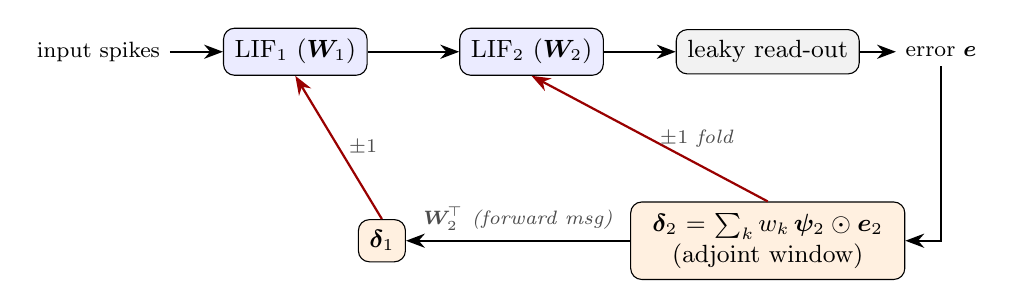
\begin{tikzpicture}[font=\footnotesize]
  \node (in) at (-2.0,0) {input spikes};
  \node[ana] (l1) at (0.5,0) {LIF$_1$ ($\bm W_1$)};
  \node[ana] (l2) at (3.5,0) {LIF$_2$ ($\bm W_2$)};
  \node[dig] (ro) at (6.5,0) {leaky read-out};
  \node (e)  at (8.7,0) {error $\bm e$};
  \draw[flow] (in) -- (l1);
  \draw[flow] (l1) -- (l2);
  \draw[flow] (l2) -- (ro);
  \draw[flow] (ro) -- (e);
  \node[jug,align=center,text width=32mm] (d2) at (6.5,-2.4) {$\bm\delta_2=\sum_{k}w_k\,\bm\psi_2\odot\bm e_2$\\ (adjoint window)};
  \node[jug] (d1) at (1.6,-2.4) {$\bm\delta_1$};
  \draw[flow] (e.south) |- (d2.east);
  \draw[flow] (d2.west) -- (d1.east) node[midway,above,lbl]{$\bm W_2^{\!\top}$ (forward msg)};
  \draw[flow,red!60!black] (d2.north) -- (l2.south) node[midway,right,lbl]{$\pm1$ fold};
  \draw[flow,red!60!black] (d1.north) -- (l1.south) node[midway,right,lbl]{$\pm1$};
\end{tikzpicture}
\caption{\textbf{The temporal credit loop, forwards-only.} Forward: input spikes $\to$ LIF stack $\to$ leaky read-out $\to$ error $\bm e$. Each layer forms its adjoint $\bm\delta_\ell=\sum_k w_k\,\bm\psi_\ell\odot\bm e_\ell$ (a windowed, tap-weighted sum of readiness-gated error, \eqref{eq:credit}); the adjoint both writes its own weights through the leaky error accumulator (the $\pm1$ fold) and is relayed to the layer below by the transpose $\bm W_\ell^{\!\top}$ --- a forward-directed message about the past, not a reverse channel. No analog signal flows backward.}
\label{fig:dataflow}
\end{figure}

\hypertarget{sec:consolidate}{%
\subsection{Consolidation, and reliability-graded
writing}\label{sec:consolidate}}

Each layer's adjoint pairs with the \emph{current} presynaptic spike
\(\bm z_{\ell-1,t}=\bm s_{\ell-1,t}\) to form the per-sample weight
gradient
\(\bm g_\ell = \sum_t \bm\delta_{\ell,t}\,\bm z_{\ell-1,t}^{\!\top}\)
(the windowing lives in the adjoint; the presynaptic term is the spike
at time \(t\)). This is written to the weights through the same jug and
fold as Part II --- another leaky accumulator, now with a threshold. The
jug integrates credit; every \(F\) samples the fold moves the weight and
resets the jug:

\begin{equation}
\bm E_\ell \mathrel{+}= \bm g_\ell, \qquad
\text{every $F$ samples:}\quad \bm W_\ell \mathrel{+}= \eta\,\operatorname{sign}(\bm E_\ell),\quad \bm E_\ell \leftarrow 0 .
\label{eq:fold}
\end{equation}

The jug is again a leaky accumulator, now at the \emph{slowest}
timescale (many samples per fold) --- the consolidation of transient
credit into a durable weight. The \(\pm1\) \textbf{sign write} of
\eqref{eq:fold} is the base rule, and on tasks whose credit is an
\emph{aggregate} it is all that is needed --- as we will see, it is what
the EEG task uses. On the GSC temporal task it is not enough, because
the per-timestep credit in \eqref{eq:credit} is a \emph{noisy sum}:
individual timesteps disagree, and a bare sign discards how
\emph{consistent} the evidence was. There we replace the sign with a
reliability-graded step --- itself two more leaky accumulators, of the
credit's mean and of its energy:

\begin{equation}
\bm m \leftarrow \beta_1 \bm m + (1-\beta_1)\,\bm E, \qquad
\bm v \leftarrow \beta_2 \bm v + (1-\beta_2)\,\bm E^{2}, \qquad
\bm W \mathrel{+}= \eta\,\frac{\bm m}{\sqrt{\bm v}+\epsilon},
\label{eq:varnorm}
\end{equation}

which scales each synapse's step by how reliably its evidence has
pointed the same way. It is self-scaling and bounded (unlike a
raw-magnitude write, which overfits), and --- crucially --- it earns its
keep \emph{only} when credit is a noisy per-timestep sum. On an
aggregate (rate-coded) credit signal it is nearly a no-op. This is not a
knob we tune per task but a mechanism with a \textbf{falsifiable
signature}, which the two benchmarks turn into a test (Sec. 6): the
write rule a task should use is \emph{predicted} by how its credit is
formed, not chosen by search.

\hypertarget{sec:readout}{%
\subsection{On-chip read-out: the second half, also
forwards-only}\label{sec:readout}}

Credit assignment in the hidden layers is only half of learning; the
classifier read-out is the other half, and on the static chip it was fit
off-line by a host least-squares step. On the temporal task we train it
on-chip by its own gradient. The read-out sees a feature vector
\(\bm f\) --- for GSC a \emph{leaky-integrated} one, \eqref{eq:prim}
once more; for EEG an aggregate spike \emph{rate} --- and updates by the
output error:

\begin{equation}
\bm e = \mathrm{onehot}(y) - \hat{\bm p}, \qquad
\bm W_f \mathrel{+}= \eta_f\, \bm e\, \bm f^{\!\top}, \qquad
\bm b_f \mathrel{+}= \eta_f\, \bm e .
\label{eq:readout}
\end{equation}

This \emph{cold} read-out (trained from scratch alongside the hidden
layers, rather than refit each epoch) both closes the gap a
periodically-refit read-out leaves and removes the host from the
read-out. It needs one accommodation --- a learning-rate bootstrap,
since a cold head must move faster than the slowly-consolidating hidden
weights to keep up --- after which both halves of learning are the same
forward, local machinery. The single fold pulse-rate that governs
consolidation (the parameter we call \(\eta\) / boss-lr) is, notably,
the \emph{same value} across both benchmarks and the earlier static
task: a transferable constant rather than a per-task setting (Sec. 7).

\hypertarget{sec:timescales}{%
\subsection{One cell, many timescales}\label{sec:timescales}}

Collecting the roles, the design is several single leaky accumulators
specialised only by their leak and input. This points to the leaky
accumulator being a fundamental primitive for hardware-constrained
neuromorphic networks of this kind:

\begin{figure}[t]
\centering
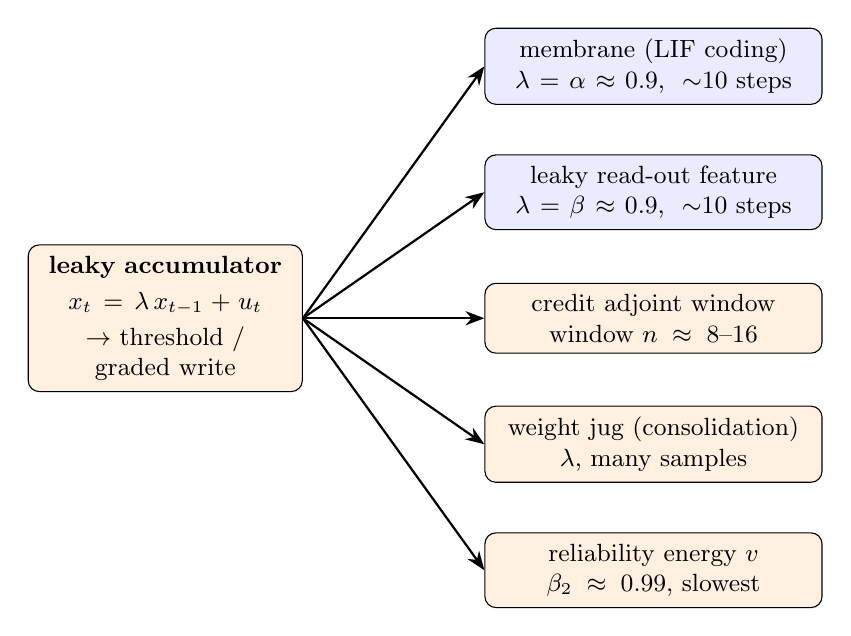
\begin{tikzpicture}[font=\footnotesize]
  \node[jug,align=center,text width=32mm] (prim) at (0,0)
    {\textbf{leaky accumulator}\\[2pt]$x_t=\lambda\,x_{t-1}+u_t$\\[2pt]$\rightarrow$ threshold / graded write};
  \node[ana,align=center,text width=40mm] (r1) at (6.2,3.2)  {membrane (LIF coding)\\ $\lambda=\alpha\approx0.9$,\ \ ${\sim}10$ steps};
  \node[ana,align=center,text width=40mm] (r2) at (6.2,1.6)  {leaky read-out feature\\ $\lambda=\beta\approx0.9$,\ \ ${\sim}10$ steps};
  \node[jug,align=center,text width=40mm] (r3) at (6.2,0)    {credit adjoint window\\ window $n\approx8$–$16$};
  \node[jug,align=center,text width=40mm] (r4) at (6.2,-1.6) {weight jug (consolidation)\\ $\lambda$, many samples};
  \node[jug,align=center,text width=40mm] (r5) at (6.2,-3.2) {reliability energy $v$\\ $\beta_2\approx0.99$, slowest};
  \foreach \r in {r1,r2,r3,r4,r5} \draw[flow] (prim.east) -- (\r.west);
\end{tikzpicture}
\caption{\textbf{One cell, five timescales.} The same leaky accumulator $x_t=\lambda x_{t-1}+u_t$ followed by a threshold or graded write, specialised only by its leak $\lambda$ and its input, performs temporal coding, leaky read-out, temporal credit, weight consolidation, and reliability grading. The unification is a finding of the search, not an imposition.}
\label{fig:primitive}
\end{figure}

\begin{longtable}[]{@{}
  >{\raggedright\arraybackslash}p{(\columnwidth - 6\tabcolsep) * \real{0.1200}}
  >{\raggedright\arraybackslash}p{(\columnwidth - 6\tabcolsep) * \real{0.2000}}
  >{\raggedright\arraybackslash}p{(\columnwidth - 6\tabcolsep) * \real{0.3600}}
  >{\raggedright\arraybackslash}p{(\columnwidth - 6\tabcolsep) * \real{0.3200}}@{}}
\caption{The same leaky-accumulator primitive \eqref{eq:prim} at five
timescales. Coding, credit, consolidation, grading and read-out are not
five mechanisms but one cell reused --- mirroring the way biology reuses
leaky integration from membrane to eligibility to
homeostasis.}\tabularnewline
\toprule\noalign{}
\begin{minipage}[b]{\linewidth}\raggedright
role
\end{minipage} & \begin{minipage}[b]{\linewidth}\raggedright
equation
\end{minipage} & \begin{minipage}[b]{\linewidth}\raggedright
leak / timescale
\end{minipage} & \begin{minipage}[b]{\linewidth}\raggedright
in the network
\end{minipage} \\
\midrule\noalign{}
\endfirsthead
\toprule\noalign{}
\begin{minipage}[b]{\linewidth}\raggedright
role
\end{minipage} & \begin{minipage}[b]{\linewidth}\raggedright
equation
\end{minipage} & \begin{minipage}[b]{\linewidth}\raggedright
leak / timescale
\end{minipage} & \begin{minipage}[b]{\linewidth}\raggedright
in the network
\end{minipage} \\
\midrule\noalign{}
\endhead
\bottomrule\noalign{}
\endlastfoot
temporal coding & \eqref{eq:lif} & \(\alpha\approx0.9\), \({\sim}10\)
steps & LIF membrane \\
leaky read-out feature & \eqref{eq:readout} & \(\beta\approx0.9\),
\({\sim}10\) steps & dendritic integration \\
temporal credit & \eqref{eq:credit} & window \(n\approx8\)--\(16\) &
eligibility trace \\
weight consolidation & \eqref{eq:fold} & many samples per fold &
synaptic tag \(\to\) consolidation \\
reliability grading & \eqref{eq:varnorm} & \(\beta_2\approx0.99\),
slowest & homeostatic scaling \\
\end{longtable}

\hypertarget{sec:hardware}{%
\section{Hardware realisation as a modular upgrade}\label{sec:hardware}}

The base of the design is unchanged from the static cell of Part II ---
the leaky jug. Because none of the temporal elements touch that base,
and because each is a version of the same primitive the chip already
implements, the temporal capability is a set of \emph{bolt-on modules},
not a redesign. Each can be included or omitted at the cell/chip/layer
level per task, and that separability is what keeps the design modular
and the key arithmetic at the neuron level, where it scales.

\begin{itemize}
\tightlist
\item
  \textbf{The LIF membrane} \eqref{eq:lif} is a leaky accumulator with a
  threshold --- the same structure as the jug, applied to activations
  rather than errors. Bypassed, the cell is the static analog MAC of
  Part II.
\item
  \textbf{The per-layer credit buffer} \eqref{eq:credit} is a small
  local first-in-first-out store (depth \(n\approx8\)--\(16\)) holding
  the recent readiness-gated error that forms the adjoint. It is
  \textbf{per-neuron, not per-synapse} --- a few hundred bits per cell
  --- and, with a \(1\)-bit sign fold, the temporal upgrade adds
  \emph{no} per-synapse digital state, preserving the base jug's
  defining property. The presynaptic spike is paired at the write, and
  the transpose that routes the adjoint down is the existing Part-II
  engine. At depth \(0\) the cell reverts to the static update.
\item
  \textbf{The tap weights} are a short causal FIR (\(w_k\) of
  \eqref{eq:credit}) over that same buffer --- a handful of shared
  coefficients per cell, not per synapse. Delta-initialised to the
  identity, the module starts as the uniform box and is trained by the
  same fold rule; it is the cheapest of the temporal additions and, on
  both tasks, the one that buys reach toward BPTT.
\item
  \textbf{The graded write} \eqref{eq:varnorm} is the one module that
  \emph{does} add per-synapse state: two slow accumulators (\(m\),
  \(v\)), several times the weight code. It is therefore
  \textbf{optional} --- it buys the last few points on the tasks that
  need it and nothing on the tasks that do not --- and its
  \(\sqrt{\cdot}\) and divide are one \emph{shared, swept} unit, as the
  jug shares its comparator, not per-synapse logic. Whether a task needs
  it at all is \emph{predicted} by Sec. 6, so it is enabled by a rule,
  not a sweep.
\item
  \textbf{The read-out} runs \textbf{per sample, not per timestep}: it
  acts on the pooled feature, so its whole cycle (score, error, gradient
  \eqref{eq:readout}, and the top-\(\bm\delta\) transpose) sits
  \emph{outside} the per-timestep loop at \(1/T\) its rate, and can be a
  plain digital MAC; the cold gradient moves it on-chip from the host.
\end{itemize}

What stays in firmware is only what stayed in Part II: the
soft-max/error scalar at the read-out. Everything else --- coding,
credit, consolidation, grading, read-out --- is the on-chip primitive. A
\emph{tiered} hardware story follows directly from the ablations of Sec.
6: the cheapest configuration (a spike-\emph{counter} read-out with a
\(1\)-bit sign write) already reaches \(0.78\) on GSC; adding the leaky
read-out, the graded write, and the learnable taps buys the rest. The
design lets the integrator choose where to sit on that curve, per task.

\hypertarget{sec:rtl}{%
\subsection{A bit-faithful RTL implementation}\label{sec:rtl}}

The modular argument is not left as a claim. We implemented the temporal
datapath in synthesisable register-transfer-level (RTL) Verilog and
verified each block \textbf{bit-exact} against a fixed-point reference
model --- the same double-build discipline Part II used for the static
jug, on the same open \(130\) nm base and simulation harness.

Every element has a verified module: the \textbf{LIF membrane} with its
readiness output \eqref{eq:lif}; the \textbf{adjoint window} that
computes the credit of \eqref{eq:credit}; the \textbf{graded write}
\eqref{eq:varnorm}, whose \(m/\sqrt{v}\) is a floor integer square-root
and divide (a look-up reciprocal-root is the area-optimal alternative);
the \textbf{cold read-out} accumulate-and-write \eqref{eq:readout}; and
the \textbf{transpose hop} \(\bm W_\ell^{\!\top}\bm\delta_\ell\) that
routes credit down a layer. For each, a fixed-point Python model is the
golden reference and a testbench checks every output bit-for-bit; the
whole set runs as a pass/fail regression in which silence counts as
failure.

Three integration levels close the loop from block to chip, each
verified \textbf{cycle-accurate}. A \textbf{single-synapse lane} wires
the forward LIF, the adjoint window, the presynaptic-spike delay, the
credit accumulator, and the graded-write fold into one streaming
datapath over a full input sequence. An \textbf{array tile} replicates
the lane across several post- and pre-synaptic units, sharing the
presynaptic lines --- the width dimension. And a \textbf{two-layer
datapath} demonstrates the paper's central claim in silicon-ready form:
the top error trains \emph{both} layers with no backward pass, because
each layer's adjoint both writes its own weights (through the jug fold)
and is routed to the layer below through the transpose. Blocks and
integration alike match their references bit-exact.

This turns ``hardware-feasible'' from an argument into a measured
result. The scope is stated plainly: the datapaths are verified at the
block, tile, and two-layer level, not yet as a full swept array;
resource \emph{sharing} --- one comparator and one square-root/divide
time-multiplexed across the array --- is an area optimisation on top of
the proven datapath, not a correctness question. Transistor-level SPICE
of the new cells and place-and-route remain, as in Part II, the
pre-silicon steps beyond this study.

\hypertarget{sec:eval}{%
\section{Evaluation on two temporal benchmarks}\label{sec:eval}}

\hypertarget{setup}{%
\subsection{Setup}\label{setup}}

We test the \emph{same} architecture on two temporal signals of opposite
character, without per-task finessing of the rule.

\textbf{Google Speech Commands (GSC)}, under the NeuroBench temporal
protocol \cite{warden2018speech, yik2024neurobench}: \(35\) keyword
classes, audio delta-modulated into spike trains of \(T=200\) timesteps,
a \([20,256,256,256]\) LIF network, and a \textbf{leaky-integrator
read-out}. The signal is sparse and event-like, and its credit is a
genuinely temporal per-timestep sum.

\textbf{THOR EEG motor imagery (EEG-MI)}: binary left/right
imagined-hand movement, \(62\) EEG channels over \(T=250\) timesteps,
decoded by a shallow spiking network with a \textbf{rate (spike-count)
read-out}. Here the class information is band \emph{power} --- a
second-order, aggregate quantity --- so the credit at a synapse is a
pooled count rather than a noisy per-step sum. The contrast with GSC is
deliberate: it is what makes the write-rule law testable rather than
asserted.

For both, the comparator is the \emph{same forward network} trained
end-to-end by full BPTT with the Adam optimiser --- the unconstrained
upper bound. The forwards-only rule and the BPTT comparator differ only
in how credit is assigned and written; the forward pass, the data, and
the read-out target are identical. We report best validation accuracy
over seeds; recipes and seeds are in the repository. The framing is
deliberately asymmetric: Adam-BPTT is not a rival to beat but the
\emph{best pure-maths result} against which a deliberately constrained
system is measured. The claim is not equality but \emph{how close a
realisable, forwards-only system gets.}

\hypertarget{speech-the-result-across-scale}{%
\subsection{Speech: the result across
scale}\label{speech-the-result-across-scale}}

\begin{longtable}[]{@{}
  >{\raggedright\arraybackslash}p{(\columnwidth - 6\tabcolsep) * \real{0.2174}}
  >{\raggedleft\arraybackslash}p{(\columnwidth - 6\tabcolsep) * \real{0.2899}}
  >{\raggedleft\arraybackslash}p{(\columnwidth - 6\tabcolsep) * \real{0.4203}}
  >{\raggedleft\arraybackslash}p{(\columnwidth - 6\tabcolsep) * \real{0.0725}}@{}}
\caption{Forwards-only vs full-BPTT on temporal GSC (leaky read-out),
across training-set size, and with the learnable-tap buffer at full
scale.}\tabularnewline
\toprule\noalign{}
\begin{minipage}[b]{\linewidth}\raggedright
training data
\end{minipage} & \begin{minipage}[b]{\linewidth}\raggedleft
forwards-only rule
\end{minipage} & \begin{minipage}[b]{\linewidth}\raggedleft
Adam (full-\(200\)-step BPTT)
\end{minipage} & \begin{minipage}[b]{\linewidth}\raggedleft
gap
\end{minipage} \\
\midrule\noalign{}
\endfirsthead
\toprule\noalign{}
\begin{minipage}[b]{\linewidth}\raggedright
training data
\end{minipage} & \begin{minipage}[b]{\linewidth}\raggedleft
forwards-only rule
\end{minipage} & \begin{minipage}[b]{\linewidth}\raggedleft
Adam (full-\(200\)-step BPTT)
\end{minipage} & \begin{minipage}[b]{\linewidth}\raggedleft
gap
\end{minipage} \\
\midrule\noalign{}
\endhead
\bottomrule\noalign{}
\endlastfoot
\(8\)k / \(12\) ep & \(0.668\) & \(0.721\) & \(0.054\) \\
\(30\)k / \(20\) ep & \(0.770\) & \(0.806\) & \(0.036\) \\
full \(84\)k / \(20\) ep & \textbf{\(0.832\)} & \textbf{\(0.881\)} &
\(0.049\) \\
full \(84\)k, \textbf{+ learnable taps} & \textbf{\(0.866\)} & \(0.881\)
& \textbf{\(0.015\)} \\
\end{longtable}

The forwards-only rule reaches \(0.832\) on the full benchmark against a
full-BPTT ceiling of \(0.881\) --- about \(94\%\) of the backpropagation
result, forwards-only, with a shallow buffer against a \(200\)-step
unroll. This headline uses the committed \emph{uniform} window; the
faithful decaying adjoint reaches the same \(0.831\), so the number
rests on the mechanism the hardware actually implements. Making the
buffer's delay \textbf{learnable} (the taps of Sec. 4.3) then adds
\(+0.032\) at full scale and \emph{stacks on} the uniform cell, reaching
\(0.866\) and narrowing the gap to Adam from \(0.049\) to \(0.015\) ---
about \(98\%\) of BPTT. The tap replaces nothing; it lets the same
buffer spend its reach where credit lies.

\hypertarget{eeg-the-same-rule-a-second-modality}{%
\subsection{EEG: the same rule, a second
modality}\label{eeg-the-same-rule-a-second-modality}}

\begin{longtable}[]{@{}lrrr@{}}
\caption{Forwards-only vs full-BPTT on THOR EEG-MI (rate read-out, \(4\)
seeds). The forwards-only rule \emph{needs} the wider window; the BPTT
comparator is indifferent to it.}\tabularnewline
\toprule\noalign{}
window depth (tap \(K\)) & forwards-only rule & Adam (full BPTT) &
gap \\
\midrule\noalign{}
\endfirsthead
\toprule\noalign{}
window depth (tap \(K\)) & forwards-only rule & Adam (full BPTT) &
gap \\
\midrule\noalign{}
\endhead
\bottomrule\noalign{}
\endlastfoot
\(K=8\) & \(0.637\) & \(0.705\) & \(0.068\) \\
\(K=16\) & \textbf{\(0.668 \pm 0.001\)} & \textbf{\(0.709 \pm 0.005\)} &
\(0.042\) \\
\end{longtable}

On EEG the forwards-only rule reaches \(0.668\) against an Adam-BPTT
ceiling of \(0.709\) (chance \(0.50\)) --- again about \(94\%\) of the
backpropagation result (\(94.1\%\)), and a third independent
confirmation of the \({\sim}94\%\) figure after EMNIST (static, Part II)
and GSC (temporal). Two features are worth drawing out. First, the
\textbf{buffer reach is load-bearing here}: extending the window from
\(K=8\) to \(K=16\) lifts the rule by \(+0.030\) while the BPTT
comparator barely moves (\(0.705\to0.709\)) --- the forwards-only rule
is the one that must \emph{reach} far enough, exactly as the composition
argument predicts, because EEG's informative timescale is longer than
speech's. Second, this task uses the \textbf{\(1\)-bit sign write}, not
the graded one, and does so by prediction rather than by choice (next
section).

\hypertarget{what-is-load-bearing-and-the-write-rule-law}{%
\subsection{What is load-bearing, and the write-rule
law}\label{what-is-load-bearing-and-the-write-rule-law}}

Two mechanisms carry the temporal result, and both are settled by
ablation rather than assertion.

\textbf{The learnable tap / buffer reach.} On GSC the learnable taps are
worth \(+0.032\) (uniform \(0.834 \to\) tapped \(0.866\)); on EEG the
window depth is worth \(+0.030\) (\(K8\to K16\)). On both, buffer
\emph{depth} is otherwise flat between \(6\) and \(12\) uniform steps,
and the uniform box matches the exact decaying adjoint over \(3\) seeds
(\(+0.004\), not significant) --- so the hardware implements the simpler
box and spends its parameters on the taps, which is where reach is
actually bought.

\textbf{The graded write, and its falsifiable law.} On GSC's leaky
read-out, replacing the graded write \eqref{eq:varnorm} with a bare sign
costs \(12\) pp (\(0.649 \to 0.770\), positive in every seed,
\(p\approx0.004\)) --- it is load-bearing. Our account is that grading
helps \emph{precisely} when credit is a noisy sum of per-timestep terms.
That account predicts it should \emph{stop} helping wherever credit is
an aggregate. Two independent controls confirm it: a \emph{rate}
read-out on GSC (which pools spikes into one count per synapse) sees
only \(+0.014\) from grading, not significant; and the \textbf{EEG
task}, whose rate read-out is aggregate by nature, sees \emph{no}
benefit and therefore uses the sign write. The single setting that
differs between our two benchmarks is thus not a tuned knob but the
output of a tested law:

\begin{longtable}[]{@{}
  >{\raggedright\arraybackslash}p{(\columnwidth - 4\tabcolsep) * \real{0.3333}}
  >{\raggedright\arraybackslash}p{(\columnwidth - 4\tabcolsep) * \real{0.2000}}
  >{\raggedright\arraybackslash}p{(\columnwidth - 4\tabcolsep) * \real{0.4667}}@{}}
\caption{The write-rule law. Whether a task needs the graded write is
predicted by how its credit is formed, and the two benchmarks fall on
opposite sides of the prediction.}\tabularnewline
\toprule\noalign{}
\begin{minipage}[b]{\linewidth}\raggedright
credit signal
\end{minipage} & \begin{minipage}[b]{\linewidth}\raggedright
example
\end{minipage} & \begin{minipage}[b]{\linewidth}\raggedright
graded write helps?
\end{minipage} \\
\midrule\noalign{}
\endfirsthead
\toprule\noalign{}
\begin{minipage}[b]{\linewidth}\raggedright
credit signal
\end{minipage} & \begin{minipage}[b]{\linewidth}\raggedright
example
\end{minipage} & \begin{minipage}[b]{\linewidth}\raggedright
graded write helps?
\end{minipage} \\
\midrule\noalign{}
\endhead
\bottomrule\noalign{}
\endlastfoot
noisy per-timestep sum & GSC, leaky read-out & \textbf{yes} (\(+0.121\),
\(p\approx0.004\)) \\
aggregate (pooled) & GSC, rate read-out & no (\(+0.014\), n.s.) \\
aggregate (pooled) & EEG-MI, rate read-out & no (sign write used) \\
\end{longtable}

\hypertarget{sec:robust}{%
\section{Robustness: one generalist cell, not a task-specific
design}\label{sec:robust}}

Of the three invariants inherited from Parts I and II --- forwards-only,
robust, asynchronous --- it is \emph{robustness} that the temporal work
most sharpens, and it is the result we most want to carry. Robustness
here means more than tolerance of device mismatch (which Part II
established, and which the coarse \(1\)-bit write and per-synapse
learning-rate spread still provide). It means a \textbf{generalist}
architecture: one cell, one credit mechanism, one forwards-only
discipline, applied to two temporal signals of opposite character
without redesign.

The evidence is that the design does \emph{not} get re-tuned per task.
GSC is deep, sparse and event-like with a leaky read-out; EEG is
shallow, continuous and power-based with a rate read-out. The forward
model, the eligibility-window credit path, the transpose routing, the
jug-and-fold consolidation, the cold on-chip read-out, and the fold
pulse-rate constant are common to both. The learnable-tap buffer is the
shared mechanism that supplies temporal reach on each. Where the tasks
differ, they differ in ways the architecture \emph{anticipates} rather
than requires hand-setting:

\begin{itemize}
\tightlist
\item
  The \textbf{write rule} (graded vs \(1\)-bit sign) is the one
  substantive difference, and it is \emph{predicted} by the write-rule
  law: GSC's noisy per-timestep credit calls for grading, EEG's
  aggregate credit does not. This is the opposite of task-specific
  finessing --- the same rule, applied, tells you which module to
  enable.
\item
  The \textbf{fold pulse-rate} is a single value transferred unchanged
  across GSC (temporal), EMNIST (static, Part II), and EEG (band-power).
  For a substrate that cannot trim per device, a transferable global
  constant with a broad tolerance plateau is exactly the property a
  generalist design needs; a knob that had to be re-found per task would
  undermine the whole approach.
\end{itemize}

We read this as the practical meaning of a hardware-first design:
because the cell is chosen to satisfy fixed physical constraints rather
than to fit one dataset, it inherits a generality that a task-optimised
network does not. The leaky accumulator is the prime component in this
because it is the one part reused everywhere --- and reuse across roles
\emph{within} a task is what makes reuse across tasks unsurprising. A
generalist edge learner does not need a new architecture for every
signal; it needs one robust primitive and a rule for where to apply it.

\hypertarget{sec:gap}{%
\section{Approaching BPTT: what the gap is, and why it is
acceptable}\label{sec:gap}}

The buffer \eqref{eq:credit} recovers the BPTT gradient \emph{direction}
closely --- an independent probe finds cosine similarity near unity ---
so it is fair to ask whether it is simply truncated BPTT wearing a
forward mask. It is not, and the distinction is physical. In the
taxonomy of online learning \cite{marschall2020unified} the buffer is a
\emph{forward-mode} (RTRL-family) approximation --- SnAp-\(n\)
\cite{menick2021snap} --- not truncated BPTT: the two converge to the
same gradient but compute it in opposite directions, and only the
forward one is realisable on this substrate. The buffer is a
\emph{per-layer, local} accumulation computed \emph{forward in time}: no
error propagates backward across layers, and no global unrolled history
is held. Its agreement with BPTT is the useful finding --- that a
shallow local eligibility trace, composed down the stack, is a good
approximation to the global gradient --- not a contradiction.

We also looked hard for the residual. Across both tasks a
\({\sim}5\)-point gap to Adam remains at the uniform-window setting (GSC
\(0.832/0.881\); EEG \(0.668/0.709\)), and we searched the write path
for it: finer per-synapse magnitude writes, a self-annealing step-size
damper, and the graded write itself all bear on \emph{how} credit is
written. None closes the gap, and the reason is instructive: the graded
write is the strongest bounded write in the family, and where it helps
(GSC) it still leaves the same residual, while where it does not (EEG) a
finer write is not the lever either. The residual is therefore not in
the \emph{magnitude} of the written credit but in its \emph{direction}
--- the forwards-only windowed adjoint computes a gradient that
approximates BPTT's but is not identical to it, by design (a bounded
forward reach in place of the full backward unroll). On GSC the
learnable taps recover most of it (to \(0.866\), \({\sim}98\%\)); on
EEG, whose credit direction is genuinely harder to form forward, more of
it remains. This is the honest boundary: a close, cheap, forward
\emph{approximation} to BPTT, not an equivalence, with a residual that
is bounded and localised rather than mysterious.

That boundary is, we think, the right one for a hardware-first design to
accept. A maths-perfect BPTT result is not physically reachable on a
forward, local, coarse substrate, and chasing the last points by adding
a backward channel or unbounded per-synapse memory would forfeit the
very properties the design exists to provide. A robust generalist that
reaches \({\sim}94\)--\(98\%\) of the backpropagation ceiling on two
unlike temporal tasks, forwards-only and with a few hundred bits of
local buffer, is the useful object. Nature does not compute a perfect
gradient either; it computes a good-enough one, locally and forward, and
so do we.

\hypertarget{sec:conclusion}{%
\section{Limitations and conclusion}\label{sec:conclusion}}

\textbf{Limitations and future work.} All results are pre-silicon
(behavioural and bit-faithful models, not a fabricated die). The
temporal rule is now characterised on two benchmarks rather than one,
which broadens the generality claim, but both are edge-scale
classification; whether the primitive's reuse transfers to larger or
more structured temporal problems is open. Two trade-offs are
characterised but left open. The \textbf{\({\sim}5\)-point gap to full
BPTT} at the uniform setting is closed to \({\sim}1.5\) points on GSC by
the learnable taps but remains wider on EEG; we have localised it to the
forward credit \emph{direction} rather than the write magnitude, but not
eliminated it. And the \textbf{graded write's per-synapse cost}: it is
the one module that adds per-synapse digital state, for the tasks the
law says need it; whether a cheaper middle ground between a \(1\)-bit
sign and full per-synapse reliability recovers most of that gain is
flagged, not resolved. The credit buffer is otherwise a truncated local
adjoint (credit outside its window is not recovered; the composition
argument that keeps it shallow is empirical, not bounded in general).

\textbf{Conclusion.} A forwards-only, hardware-constrained learning rule
can assign temporal credit on real spiking benchmarks, reaching about
\(94\%\) of full-BPTT accuracy --- up to \({\sim}98\%\) with a
learnable-delay buffer --- with a shallow local buffer and no backward
pass. The economy of the result is one of its points: coding, credit,
consolidation, reliability grading, and read-out are not separate
mechanisms but one leaky-accumulator cell reused at several timescales,
and that cell is a modular addition to the static chip rather than a new
design. But the point we most want to leave is \emph{robustness}. The
same architecture handles two temporal signals of opposite character ---
sparse audio spikes and continuous EEG power --- without task-specific
redesign, and the single setting that differs between them is predicted
by a falsifiable law rather than tuned. The unification of roles was not
imposed but found; the generalisation across tasks was tested, not hoped
for; and both, we read, are properties of building from a robust
primitive under fixed hardware constraints --- and of the biology that
builds under the same ones.

\hypertarget{acknowledgements}{%
\section*{Acknowledgements}\label{acknowledgements}}
\addcontentsline{toc}{section}{Acknowledgements}

Architectural direction and design decisions are the author's.
Simulators and experiments were implemented with Claude Code
\cite{anthropic2025claudecode} (Opus and Fable models), whose
contribution was the rate at which the mechanism space could be searched
and characterised.


\bibliographystyle{IEEEtran}
\bibliography{refs}
\end{document}
